%--------- プリアンブル ---------%
\documentclass[dvipdfmx, 12pt]{beamer}
\usepackage{bxdpx-beamer}               % dvipdfmx には必要
\usepackage{pxjahyper}                  % しおりの文字化けを防ぐ
\usepackage{minijs}                     % フォントメトリックをまともに

% パッケージ
\usepackage{otf}                        % 日本語フォント
\usepackage{graphicx}                   % 画像取り込み(オプション不要)
\usepackage{multicol}                   % 段組みにする
\usepackage{tikz}                       % 汎用的な描画
\usepackage{listings}                   % ソースコード貼り付け


\renewcommand{\kanjifamilydefault}{\gtdefault}

\hypersetup{
    setpagesize=false,
    bookmarksnumbered=true,
    bookmarksopen=true,
    colorlinks=true,
    linkcolor=blue!75,
    urlcolor=teal!60
}

\usetikzlibrary{arrows.meta, shapes.callouts}

\tikzset{callout/.style={rectangle callout, rounded corners, white, fill=red!75, minimum height=30pt}}
\tikzset{probrem/.style={rectangle, white, fill=red!75, text centered, font=\huge, minimum width=24zw}}

\tikzset{block/.style={rectangle, rounded corners, draw, text centered, minimum height=20pt}}
\tikzset{progress/.style={block, fill=cyan!12}}
\tikzset{progress10/.style={progress, minimum width=10zw}}
\tikzset{progress20/.style={progress, minimum width=20zw}}
\tikzset{success/.style={block, fill=magenta!12, minimum width=10zw}}
\tikzset{failure/.style={block, red, fill=red!12}}

\lstset{
    basicstyle=\ttfamily\footnotesize,
    commentstyle=\color[rgb]{0.0,0.6,0.0},
    backgroundcolor=\color[rgb]{0.95,0.95,0.92},
    columns=[l]{fullflexible},
    frame=tlBR,
    framesep=5pt,
    lineskip=-0.3ex,
    breaklines=true,
    breakatwhitespace=false,
    keepspaces=true,
    showspaces=false,
    showstringspaces=false,
    showtabs=false
}

\colorlet{number}{green!60!black}
\definecolor{bracket}{RGB}{20,100,175}

\lstdefinelanguage{json}{
    keywords={null, true, false},
    keywordstyle=\color{blue!60!black},
    literate=
       *{0}{{{\color{number}0}}}{1}
        {1}{{{\color{number}1}}}{1}
        {2}{{{\color{number}2}}}{1}
        {3}{{{\color{number}3}}}{1}
        {4}{{{\color{number}4}}}{1}
        {5}{{{\color{number}5}}}{1}
        {6}{{{\color{number}6}}}{1}
        {7}{{{\color{number}7}}}{1}
        {8}{{{\color{number}8}}}{1}
        {9}{{{\color{number}9}}}{1}
        {\{}{{{\color{bracket}{\{}}}}{1}
        {\}}{{{\color{bracket}{\}}}}}{1}
        {[}{{{\color{bracket}{[}}}}{1}
        {]}{{{\color{bracket}{]}}}}{1},
    numbers=left,
    numberstyle=\scriptsize,
    firstnumber=1,
    stepnumber=1,
    numbersep=9pt
}


% 設定情報
\usetheme[]{metropolis}
\usefonttheme{professionalfonts}

\setbeamercolor{normal text}{bg=white}
\setbeamercolor{enumerate item}{fg=blue!75}
\setbeamercolor{description item}{fg=blue!75}

\setbeamertemplate{caption}{\raggedright\insertcaption\par}
\setbeamertemplate{navigation symbols}{}

\setbeamercolor{footline}{fg=red!75}
\setbeamertemplate{footline}[frame number]
\setbeamerfont{footline}{series=\bfseries}

\AtBeginSection[]{
    \begin{frame}{目次}
        \tableofcontents[currentsection]
    \end{frame}
}


% 属性情報
\title{Dockerfileの開発を支援する\\インタラクティブツールの提案}
\author{稲田 司}
\institute{\small 鵜林・亀井研究室}
\date{\today}


% 変数定義
\newlength{\mytotalwidth}
\newlength{\mycolumnwidth}
\mytotalwidth=\dimexpr\linewidth-5mm
\mycolumnwidth=\dimexpr\mytotalwidth-5mm


%--------- スライド ---------%
\begin{document}


\frame{\maketitle}

\begin{frame}{目次}
    \tableofcontents
\end{frame}


%1 導入
\section{導入}

\begin{frame}{Dockerとは何か?}
    アプリケーション実行環境を構築,共有,起動するための\\ソフトウェアプラットフォーム.

    \begin{figure}
        \centering
        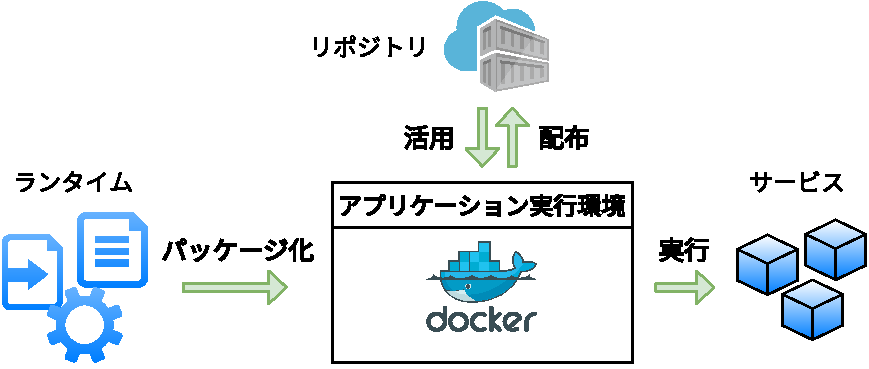
\includegraphics[width=\linewidth]{img/docker.pdf}
    \end{figure}
\end{frame}


\begin{frame}{Dockerfileとは何か?}
    Dockerにおいて,
    \begin{description}
        \item[イメージ] OSやアプリケーションのテンプレート
        \item[コンテナ] イメージから生成するアプリケーション実行環境
    \end{description}

    Dockerfileは,イメージ構築を自動化する一連の命令列が\\記載されたテキストファイル.

    \begin{columns}[totalwidth=\mytotalwidth]
        \begin{column}[T]{0.05\mycolumnwidth}
        \end{column}
        \begin{column}[T]{0.25\mycolumnwidth}
            \begin{figure}
                \centering
                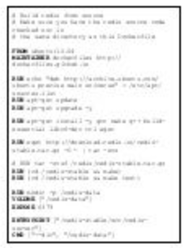
\includegraphics[height=60pt]{img/_dockerfile.png}
                \caption{Dockerfile}
            \end{figure}
        \end{column}
        \begin{column}[T]{0.1\mycolumnwidth}
            \vskip2.0zh
            \centerline{build}
            \centerline{$\longrightarrow$}
        \end{column}
        \begin{column}[T]{0.3\mycolumnwidth}
            \begin{figure}
                \centering
                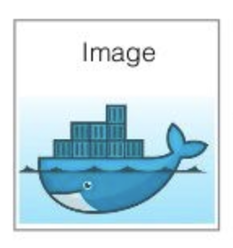
\includegraphics[height=60pt]{img/_image.png}
                \caption{イメージ}
            \end{figure}
        \end{column}
        \begin{column}[T]{0.1\mycolumnwidth}
            \vskip1.0zh
            \centerline{run}
            \centerline{$\longrightarrow$}
            \centerline{\footnotesize (commit)}
            \centerline{$\dashleftarrow$}
        \end{column}
        \begin{column}[T]{0.3\mycolumnwidth}
            \begin{figure}
                \centering
                
\includegraphics[height=60pt]{img/_container.png}
                \caption{コンテナ}
            \end{figure}
        \end{column}
    \end{columns}
\end{frame}
%2 背景と目的
\section{背景と目的}

\begin{frame}{イメージが抱える課題とその解決手法}
    \begin{multicols}{2}
        \begin{list}{}{\setlength{\itemsep}{1.0zh}}
            \setlength{\itemindent}{-3.0zw}
            \item ビルド時間の短縮
            \item イメージサイズの削減
            \item イメージ分析
            \item サイバー攻撃への対策
            \item 同一性の確認
            \item 再現性の確保
            \item イメージ開発の効率化
            \item 保守性の確保
        \columnbreak
        \setlength{\itemindent}{-4.6zw}
            \begin{onlyenv}<2->
                \item[→] キャッシュの利用,BuildKit
                \item[→] マルチステージビルド,Slim
                \item[→] dive,dlayer
                \item[→] Distrolessイメージ,BuildKit
                \item[→] ハッシュによる確認,イメージ署名
                \item[→] ?
            \end{onlyenv}
            \begin{onlyenv}<2-3>
                \item[→] ?
                \item[→] ?
            \end{onlyenv}
            \begin{onlyenv}<4>
                \item[→] \textcolor{orange}{インタラクティブツール}
                \item[→] \textcolor{orange}{リファクタリング・最適化の機能}
            \end{onlyenv}
        \end{list}
    \end{multicols}

    \begin{onlyenv}<3>
        \begin{tikzpicture}[remember picture]
            \useasboundingbox (0.0, 0.0);
            \begin{scope}[shift={(current page.south west)}]
                \node[callout, callout absolute pointer={(6.4, 1.9)}] at (9.6, 1.5) {提案ツールで解決したい};
                \node[callout, callout absolute pointer={(6.4, 0.9)}] at (9.6, 1.5) {提案ツールで解決したい};
            \end{scope}
        \end{tikzpicture}
    \end{onlyenv}
\end{frame}
%3 提案ツールの特長
\section{提案ツールの特長}

\begin{frame}{なぜ,イメージ開発の効率化が必要なのか?}
    下のギャップが,開発を非効率にしている.
    \begin{description}[labelwidth=6.0zw]
        \item[イメージ開発] Dockerfileを作成する.
        \item[動作確認] コンテナ内で行う.
    \end{description}

    \vskip1.0zh
    現状の動作確認の手段
    \begin{enumerate}
        \item 同じベースイメージから起動したコンテナを使う.
        \item 開発中のDockerfileから逐一起動するコンテナを使う.
    \end{enumerate}

    \vskip0.5zh
    どちらも,\textcolor{red!75}{問題あり}.
\end{frame}


\begin{frame}{同じベースイメージから起動したコンテナで\\動作確認しながら,Dockerfileを開発する}
    目的の環境構築とDockerfileの編集作業を同時進行させる.

    → \textcolor{red!75}{開発者の負担が大きい}
    \vskip1.5zh

    \begin{figure}
        \centering
        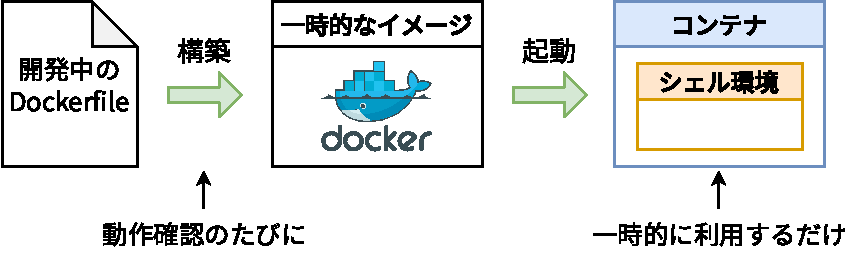
\includegraphics[width=\linewidth]{img/method1.pdf}
    \end{figure}
\end{frame}


\begin{frame}{開発中のDockerfileから逐一起動するコンテナで\\動作確認しながら,Dockerfileを開発する}
    Dockerfileを修正する度に,一時的なイメージを構築する.

    → \textcolor{red!75}{待ち時間が発生する}
    \vskip1.5zh

    \begin{figure}
        \centering
        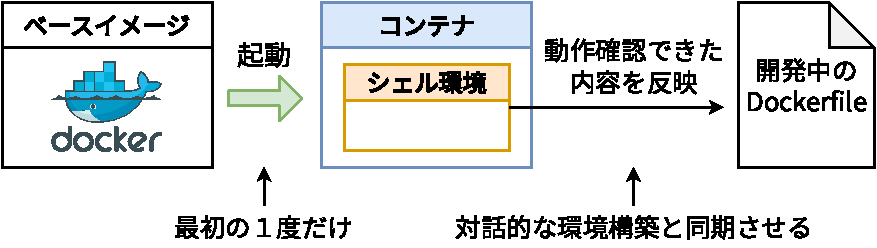
\includegraphics[width=\linewidth]{img/method2.pdf}
    \end{figure}
\end{frame}


\begin{frame}{提案ツールを用いて,Dockerfileを開発すると}
    \begin{figure}
        \centering
        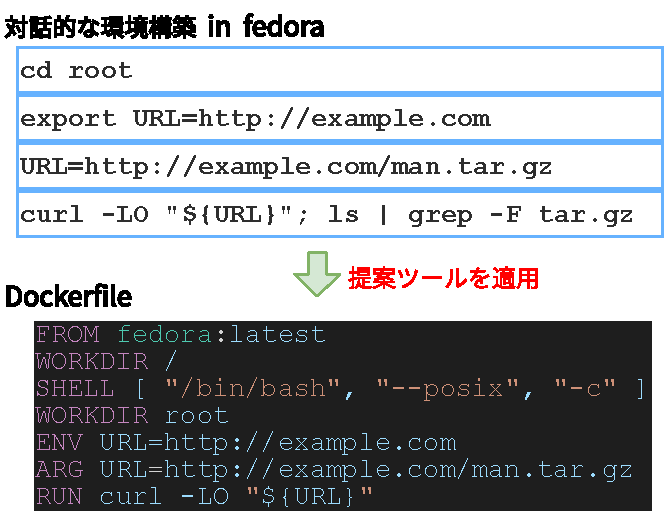
\includegraphics[width=0.95\linewidth]{img/outline.pdf}
    \end{figure}
\end{frame}


\begin{frame}{提案ツールの特長}
    Dockerfileの効率的な開発手法が必要.
    \vskip0.5zh

    \hskip3.0zw
    {\huge $\Downarrow$}
    \vskip0.5zh

    \textcolor{blue!75}{インタラクティブツールとしての側面}

    ユーザがコンテナ内で動作確認しながら環境構築することで,
    \textcolor{red!75}{自動的に}Dockerfileを生成してくれる.
\end{frame}


\begin{frame}{これだけでは優れたDockerfileにはならない}
    \begin{figure}
        \centering
        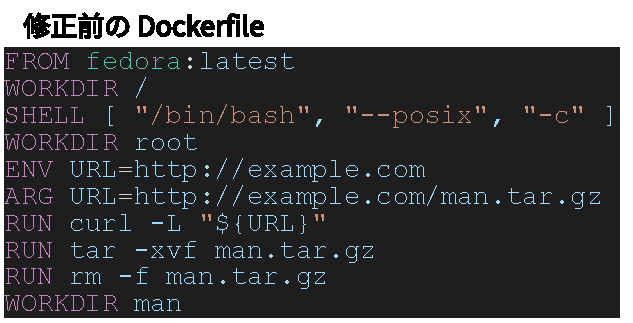
\includegraphics[width=1.02\linewidth]{img/optimize1.pdf}
    \end{figure}

    \begin{tikzpicture}[remember picture]
        \useasboundingbox (0.0, 0.0);
        \begin{scope}[shift={(current page.south west)}]
            \only<2>{\node[probrem] at (6.4, 4.0) {見づらい};}

            \begin{onlyenv}<3>
                \node[callout, callout absolute pointer={(5.6, 4.8)}] at (8.6, 6.6) {絶対パス指定の方がいい};
                \node[callout, callout absolute pointer={(6.4, 3.4)}] at (9.0, 2.0) {集約した方がいい};
                \node[callout, callout absolute pointer={(7.2, 4.2)}] at (9.0, 2.0) {集約した方がいい};
            \end{onlyenv}
        \end{scope}
    \end{tikzpicture}
\end{frame}


\begin{frame}{Dockerfileのリファクタリング・最適化を行ってみる}
    \begin{figure}
        \centering
        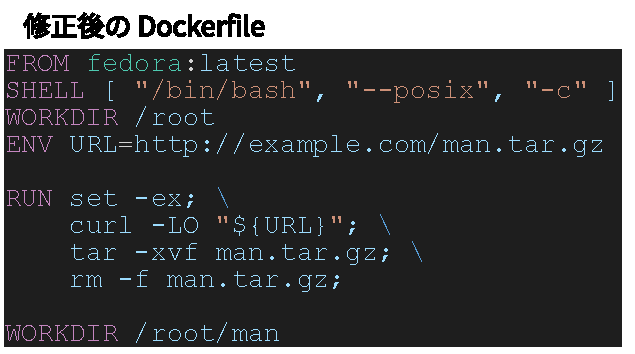
\includegraphics[width=1.02\linewidth]{img/optimize2.pdf}
    \end{figure}
\end{frame}


\begin{frame}{提案ツールの特長}
    \textcolor{blue!75}{インタラクティブツールとしての側面}

    ユーザがコンテナ内で動作確認しながら環境構築することで,
    \textcolor{red!75}{自動的に}Dockerfileを生成してくれる.

    \vskip1.0zh
    \textcolor{blue!75}{リファクタリング・最適化の機能}

    上のようにして生成したDockerfileに,ベストプラクティスに基づいたリファクタリング・最適化を行うことができる.
\end{frame}
%4 簡単な使い方
\section{簡単な使い方}

\begin{frame}[fragile]{手順 1/4\\「提案ツールのソースコードを取得する」}
    提案ツールの\href{https://github.com/posl/dit}{\textcolor{teal!60}{リポジトリ}}をクローンする.
    \vskip2.0zh

    実行例
\begin{lstlisting}[]
URL=https://github.com/posl/dit.git
git clone --depth 1 "${URL}"
\end{lstlisting}

\end{frame}


\begin{frame}[fragile]{手順 2/4\\「開発用のコンテナを起動し,開発を開始する」}
    開発用のディレクトリを設定しながら,\textcolor{orange}{exec.sh}を実行する.\\
    実行後は,指定したベースイメージに\textcolor{orange}{bash}で入った状態.

    \begin{figure}
        \centering
        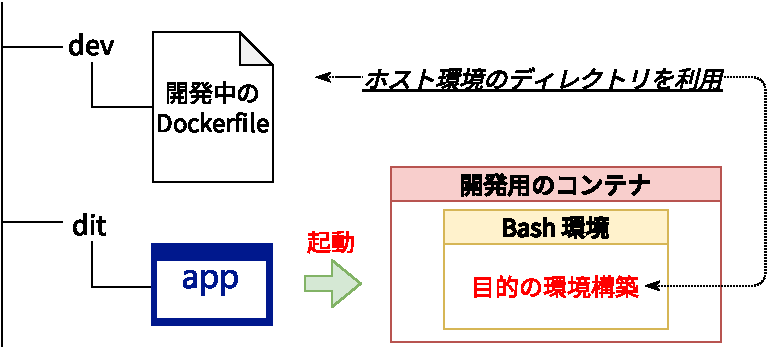
\includegraphics[width=\linewidth]{img/usage1.pdf}
    \end{figure}
\end{frame}


\begin{frame}{手順 3/4\\「動作確認しながら,目的の環境構築を行う」}
    コンテナ内で動作確認しながら,環境構築することで,\\
    それと同時に,\textcolor{orange}{自動的に}Dockerfileが作られていく.

    \begin{figure}
        \centering
        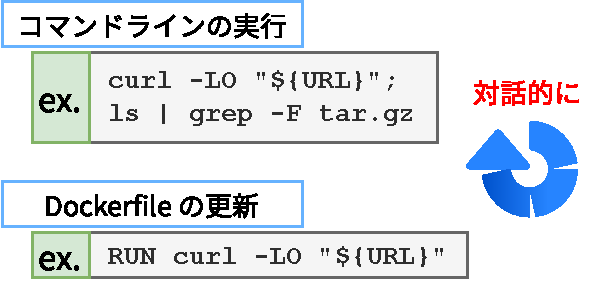
\includegraphics[width=0.8\linewidth]{img/usage2.pdf}
    \end{figure}
\end{frame}


\begin{frame}{手順 4/4\\「Dockerfileを完成させる」}
    次の処理は,提案ツールの機能を使う.
    \begin{description}[labelwidth=6.0zw]
        \item[dit package] パッケージのインストール
        \item[dit copy] ホスト環境からのファイルのコピー
        \item[dit optimize] Dockerfileのリファクタリング・最適化
    \end{description}

    \vskip2.0zh
    最後に,Dockerfileのリファクタリング・最適化を行う.

    これで,目的のDockerfileが完成する.
\end{frame}
%5 主な機能
\section{主な機能}

\newcommand{\MyFunctionTable}[4]{
    \begin{frame}{機能要件}
        \begin{enumerate}
            \setbeamercovered{dynamic}
            \setlength{\itemsep}{0.8zh}
            \item<#1> 任意のコマンドラインを実行するたびに,その必要性を判断して,対応する命令をDockerfileに追加する機能
            \item<#2> CUI上でDockerfileを編集する機能
            \item<#3> ベストプラクティスに基づいて,作成されたDockerfileのリファクタリング・最適化を行う機能
            \item<#4> Dockerfileの開発を任意のタイミングで中断・再開できるようにする機能
        \end{enumerate}
    \end{frame}
}

\MyFunctionTable{1}{1}{1}{1}
\MyFunctionTable{1}{0}{0}{0}


\begin{frame}[fragile]{機能1\\「任意のコマンドラインを実行するたびに処理を行う」}
    Bashのシェル変数PROMPT\_COMMANDを使用する.
    \vskip2.0zh

    使用例
\begin{lstlisting}[language=sh]
# log each time the shell prompt is updated
PROMPT_COMMAND='mylog > "/tmp/$(date -Ins)"'
\end{lstlisting}

\end{frame}


\begin{frame}{機能1\\「変換仕様により,コマンドの反映の要否を判断する」}
    \begin{figure}
        \centering
        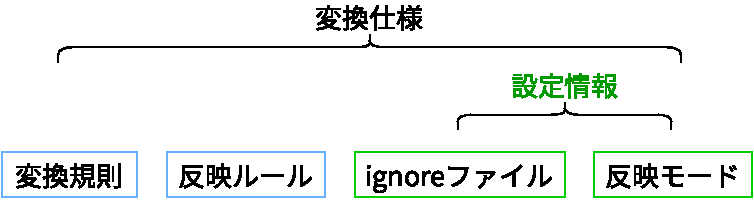
\includegraphics[width=0.92\linewidth]{img/terms.pdf}
    \end{figure}

    \small
    \begin{table}[h]
        \centering
        \begin{tabular}{c|l}
            変換仕様 & \multicolumn{1}{c}{概要} \\
            \hline\hline
            変換規則 & コマンドとDockerfileの命令を対応づける \\
            反映ルール & 構文情報からコマンドの反映の要否を決定 \\
            ignoreファイル & 反映しないコマンドとその条件を記述 \\
            反映モード & 反映ルール・ignoreファイルの使い方を変更 \\
        \end{tabular}
    \end{table}
\end{frame}


\begin{frame}{機能1 変換規則の一覧}
    \small
    \begin{table}[h]
        \centering
        \begin{tabular}{c|c|l}
            変換前 & 変換後 & \multicolumn{1}{c}{備考} \\
            \hline\hline
            cd & WORKDIR命令 & 作業ディレクトリが変更された場合 \\
            pushd & & \\
            popd & & \\
            \hline
            代入文 & ARG命令 & コマンド実行環境を変更する場合 \\
            declare & & 左のコマンド以外には未対応 \\
            typeset & & \\
            readonly & & \\
            printf & & \\
            \hline
            export & ENV命令 & コマンド実行環境を変更する場合 \\
            & & ``declare -x''はARG命令に変換する \\
            \hline
            それ以外 & RUN 命令 & 複数に変換されることはない\\
        \end{tabular}
    \end{table}
\end{frame}


\begin{frame}{機能1 デフォルトの反映ルール(一部抜粋)}
    \small
    \begin{table}[h]
        \centering
        \begin{tabular}{c|l}
            Bashの構文 & \multicolumn{1}{c}{反映ルール} \\
            \hline\hline
            単純なコマンド & 出力のリダイレクションを含む場合は反映する \\
            算術式 & letに対するignoreファイルの設定を使う \\
            条件式 & 単独で使われた場合は反映しない \\
            パイプライン & 反映するコマンドより左にあるものは反映する \\
            条件付きリスト & 反映するコマンドを含む場合,まとめて反映する \\
            その他のリスト & 各コマンドの反映の要否を個別に決定する \\
        \end{tabular}
    \end{table}

    \vskip1.0zh
    \textreferencemark 後述の反映モードの設定により,内容が少し変動する.
\end{frame}


\begin{frame}[fragile]{機能1 ignoreファイルの例}
    反映しないコマンドとその条件を記述する.
\begin{lstlisting}[language=json]
{
    "ls": null,
    "dir": "ls",
    "wget": {
        "short_opts": "O:",
        "long_opts": {
            "output-document": 1
        },
        "optargs": {
            "output-document": "O",
            "O": [
                "-"
            ]
        },
        "detect_anymatch": true
    }
}
\end{lstlisting}

\end{frame}


\begin{frame}{機能1 反映モードの一覧}
    \begin{description}
        \item[no-reflect] Dockerfileに命令を追加しない
        \item[strict] 処理の流れに影響しない部分は特別視しない
        \item[normal] 処理のまとまりを考え,反映の要否を変更する
        \item[simple] 単純なコマンド\footnote{Bashの基本構文.}以外はそのまま反映する
        \item[no-ignore] 実行されたコマンドラインは必ず反映する
    \end{description}

    \vskip1.0zh
    strictとnormalの違い(例:条件実行の``left \&\& right'')
    \begin{description}
        \item[strict] 左のコマンドだけを反映する可能性がある
        \item[normal] ひとまとめに反映するか,全く反映しないか
    \end{description}
\end{frame}


\newcommand{\MyConvertExample}[2]{
    \begin{frame}{機能1 変換処理の#2}
        \begin{figure}
            \centering
            \includegraphics[width=\linewidth]{img/convert#1.pdf}
        \end{figure}
    \end{frame}
}

\MyConvertExample{1}{流れ}
\MyConvertExample{2}{実行例 1/3}
\MyConvertExample{3}{実行例 2/3}
\MyConvertExample{4}{実行例 3/3}




\MyFunctionTable{0}{1}{0}{0}


\begin{frame}{機能2\\「ホスト環境からファイルをコピーする」}
    \textcolor{blue!75}{\large dit copy}

    \hskip1.0zw
    ホスト環境からコンテナ内へのファイルのコピーを行い,その内容をCOPY・ADD命令としてDockerfileに反映する.
    \vskip2.0zh

    このコマンドを使うと,
    \begin{itemize}
        \item COPY命令とcpコマンドの仕様の違いを意識せず済む.
        \item ADD命令のtar展開機能を利用できる.
    \end{itemize}
\end{frame}


\begin{frame}{機能2\\「パッケージをインストールする」}
    \textcolor{blue!75}{\large dit package}

    \hskip1.0zw
    最適化された形式で,パッケージのインストールを行い,その内容をRUN命令としてDockerfileに反映する.
    \vskip2.0zh

    このコマンドを使うと,
    \begin{itemize}
        \item イメージサイズの削減に効果的な方法で実行される.
        \item パッケージマネージャの違いをあまり意識せず済む.
    \end{itemize}
\end{frame}


\begin{frame}[fragile]{機能2\\「Dockerfileに命令を追加する」}
    \textcolor{blue!75}{\large dit reflect}

    \hskip1.0zw
    各種ログを取りながら,Dockerfileに命令を追加する.
    \vskip1.0zh
    実行例

\begin{lstlisting}[language=sh]
# reflects the contents of `./instr.txt' in Dockerfile
dit reflect -d instr.txt
\end{lstlisting}

\begin{lstlisting}[language=sh]
# reflects the input contents as they are in Dockerfile
dit reflect -dp -
\end{lstlisting}

\end{frame}


\begin{frame}[fragile]{機能2\\「Dockerfileから指定した行を削除する」}
    \textcolor{blue!75}{\large dit erase}

    \hskip1.0zw
    条件にマッチする行を,Dockerfileから削除する.
    \vskip1.0zh
    実行例

\begin{lstlisting}[language=sh]
# deletes the lines added just before from Dockerfile
dit erase -d
\end{lstlisting}

\begin{lstlisting}[language=sh]
# deletes all LABEL instructions from Dockerfile
dit erase -diy -E '^LABEL[[:space:]]'
\end{lstlisting}

\end{frame}




\MyFunctionTable{0}{0}{1}{0}


\begin{frame}{機能3\\「Dockerfileのリファクタリング・最適化を行う」}
    \textcolor{blue!75}{\large dit optimize}

    \hskip1.0zw
    下書きのDockerfileから,完成版のDockerfileを生成する.
    \vskip1.0zh

    処理内容
    \begin{itemize}
        \item 各命令に特有のリファクタリング
        \item 順序に依存しない命令の並べ替え
        \item 連続する同系統の命令列に対する最適化
        \item 環境の整合性を保つために必須の集約処理
    \end{itemize}
\end{frame}


\begin{frame}{機能3 リファクタリング・最適化の実行例 1/3}
    \vskip2.0zh
    \begin{figure}
        \centering
        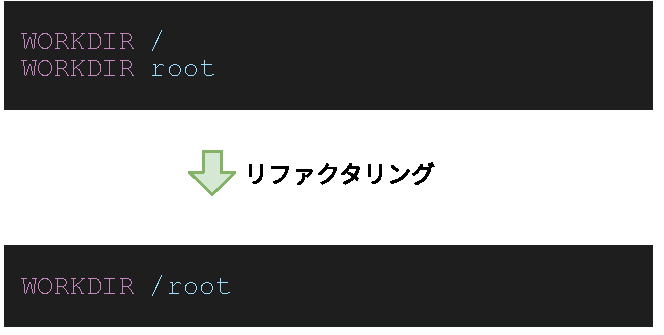
\includegraphics[width=\linewidth]{img/optimize3.pdf}
    \end{figure}

    \begin{tikzpicture}[remember picture]
        \useasboundingbox (0.0, 0.0);
        \begin{scope}[shift={(current page.south west)}]
            \begin{onlyenv}<2>
                \node[callout, callout absolute pointer={(5.6, 6.4)}] at (8.8, 6.4) {起点となる絶対パスが必要};
            \end{onlyenv}
        \end{scope}
    \end{tikzpicture}
\end{frame}


\begin{frame}{機能3 リファクタリング・最適化の実行例 2/3}
    \vskip2.0zh
    \begin{figure}
        \centering
        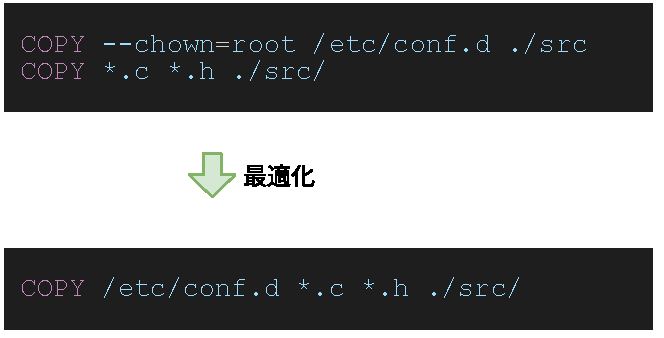
\includegraphics[width=\linewidth]{img/optimize4.pdf}
    \end{figure}

    \begin{tikzpicture}[remember picture]
        \useasboundingbox (0.0, 0.0);
        \begin{scope}[shift={(current page.south west)}]
            \begin{onlyenv}<2>
                \node[callout, callout absolute pointer={(6.4, 4.3)}] at (9.2, 4.3) {連続する命令列にのみ};
            \end{onlyenv}
        \end{scope}
    \end{tikzpicture}
\end{frame}


\begin{frame}{機能3 リファクタリング・最適化の実行例 3/3}
    \vskip0.7zh
    \begin{figure}
        \centering
        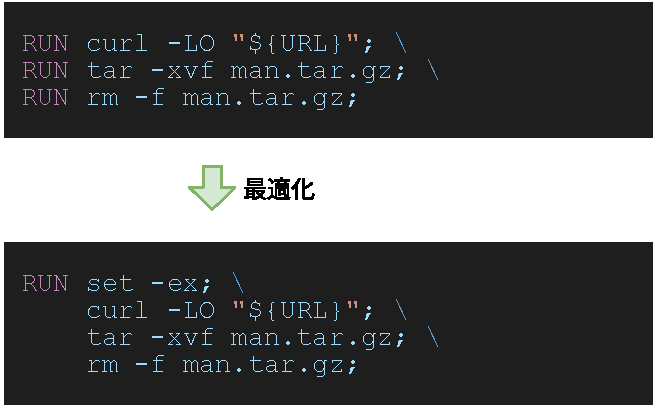
\includegraphics[width=\linewidth]{img/optimize5.pdf}
    \end{figure}

    \begin{tikzpicture}[remember picture]
        \useasboundingbox (0.0, 0.0);
        \begin{scope}[shift={(current page.south west)}]
            \begin{onlyenv}<2>
                \node[wordbox] at (10.2, 3.6) {環境の整合性を保つ};
                \node[wordbox] at (10.2, 2.4) {意味のまとまりとなる};
                \node[wordbox] at (10.2, 1.6) {イメージサイズ削減};

                \draw[white, line width=1.5pt]
                    (10.20, 2.85) -- (10.20, 3.15)
                    (10.05, 3.00) -- (10.35, 3.00);
            \end{onlyenv}
        \end{scope}
    \end{tikzpicture}
\end{frame}



\MyFunctionTable{0}{0}{0}{1}


\begin{frame}{機能4\\「Dockerfileの開発を中断・再開できるようにする」}
    コマンドラインの実行履歴を保持する,\textcolor{orange}{履歴ファイル}\\を導入することで実現する.

    \vskip1.0zh
    \begin{description}
        \setlength{\itemsep}{1.0zh}
        \setlength{\leftskip}{-1.0zw}
        \item[開発中] Dockerfileと同じように履歴ファイルを編集する.
        \item[再開時] 履歴ファイルを実行して,環境を再現する.
    \end{description}
\end{frame}
%6 まとめ
\section{まとめ}

\begin{frame}{まとめ}
    背景
    \begin{itemize}
        \setlength{\itemsep}{0.8zh}
        \item Dockerfileを効率的に開発するためのツールがない.
        \item Dockerfileのリファクタリング・最適化ツールがない.
    \end{itemize}

    \vskip2.0zh
    提案ツール
    \begin{itemize}
        \setlength{\itemsep}{0.8zh}
        \item コンテナ内のBash環境で,対話的に作業する.
        \item 動作確認に専念して,Dockerfileを開発できる.
        \item リファクタリング・最適化後のDockerfileが得られる.
    \end{itemize}
\end{frame}


\end{document}